\section{Introduction}
\label{sec:introduction}
Fault tolerance inferred from a neural endpoint can depend on which fault cohorts, observation durations and feedback laws enter the assessment. Preserved command transmission can coexist with elevated activity or failed behavior. The adult \emph{Drosophila} wiring diagram\cite{dorkenwald2024neuronal,lin2024network} and an executable spiking model\cite{shiu2024drosophila} provide an anatomically constrained substrate for quantifying this dependence. Biological wiring supplies a structural prior without validating a simplified controller's reliability.

We study software perturbations of a 138{,}639-neuron leaky integrate-and-fire (LIF) model, driving LC4/LPLC2 visual neurons and reading eight descending neurons (Fig.~\ref{fig:system}). Five families alter weights, delete weighted connection rows or silence neuronal outputs. These experiments specify neither hardware-resource mapping nor biological resilience.

\begin{figure}[t]
\centering
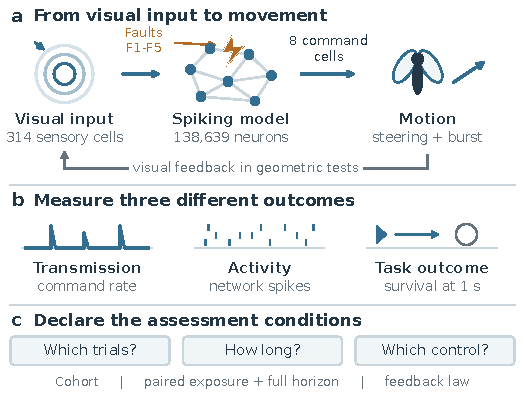
\includegraphics[width=\columnwidth]{figs/assessment_overview.pdf}
\caption{Assessment overview. (a) Model flow with visual feedback in geometric tests. (b) Distinct transmission, activity and bounded task endpoints. (c) Required assessment conditions. Icons and traces are schematic; Supplementary Fig.~S8 retains mapped wiring.}
\label{fig:system}
\end{figure}

The contribution is empirical: we quantify how assessment choices change the interpretation of fault effects in this model. Archive reanalysis holds observations fixed while varying cohort and exposure definitions; prospective tests cross two frozen control laws with healthy, 25\%-deletion and 50\%-deletion networks. Paired task loss separates fault effects from baseline controller success. Duration matching, complete trajectories and endpoint separation are established evaluation practices, not new algorithms.\footnote{Review package: \texttt{assessment-v8}, including \texttt{supplement.pdf} and reproducible paired analyses. Repository: \url{https://github.com/Scophield/drosophila-fault-injection}; this local revision is not yet published there.}
